% !TEX root = Projektdokumentation.tex

 \section{Kostenvoranschlag}
 Das Projekt läuft im Rahmen der Studienarbeit. Diese sieht einen Personenaufwand von 240 Stunden pro Person vor, was bei einer 2-Personen-Gruppe einen Aufwand von 480 Stunden macht. 
 Der Projektrahmen ist das Herbstsemester 2016, welches vom 19.09 - 23.12.2016 dauert und somit 14 Wochen umfasst. Es ist damit ein durchschnittlicher Wochenaufwand von 17 Stunden pro Person vorgesehen.
 
 
 \section{Zeitliche Planung}
 
 \subsection{Phasen / Iterationen}
 Das Projekt ist in die Phasen Inception, Elaboration, Construction und Transition aufgeteilt. Die Inception-Phase hat bereits in der Woche vor dem Semesterbeginn stattgefunden. Die restlichen Phasen sind, wie in der Grafik auf der nächsten Seite ersichtlich, über das Herbstsemesters 2017 verteilt.
 
 Zu Beginn war die Fertigstellung des Prototyp für Woche 8 geplant. Wie bei der Besprechung der neuen Mockups festgestellt, mussten jedoch noch grundlegende Konzepte überarbeitet werden. Deshalt wurde der Meilenstein 'Prototyp' sowie der damit zusammenhängende Meilenstein 'Usability-Tests' um 1 Woche nach hinten verschoben. Die Tests werden anfangs Woche durchgeführt, wodurch noch knapp 3 Wochen Implementation verbleiben, um auf kleinere Änderungen durch die Tests zu reagieren und diese im Code umzusetzen.
 
 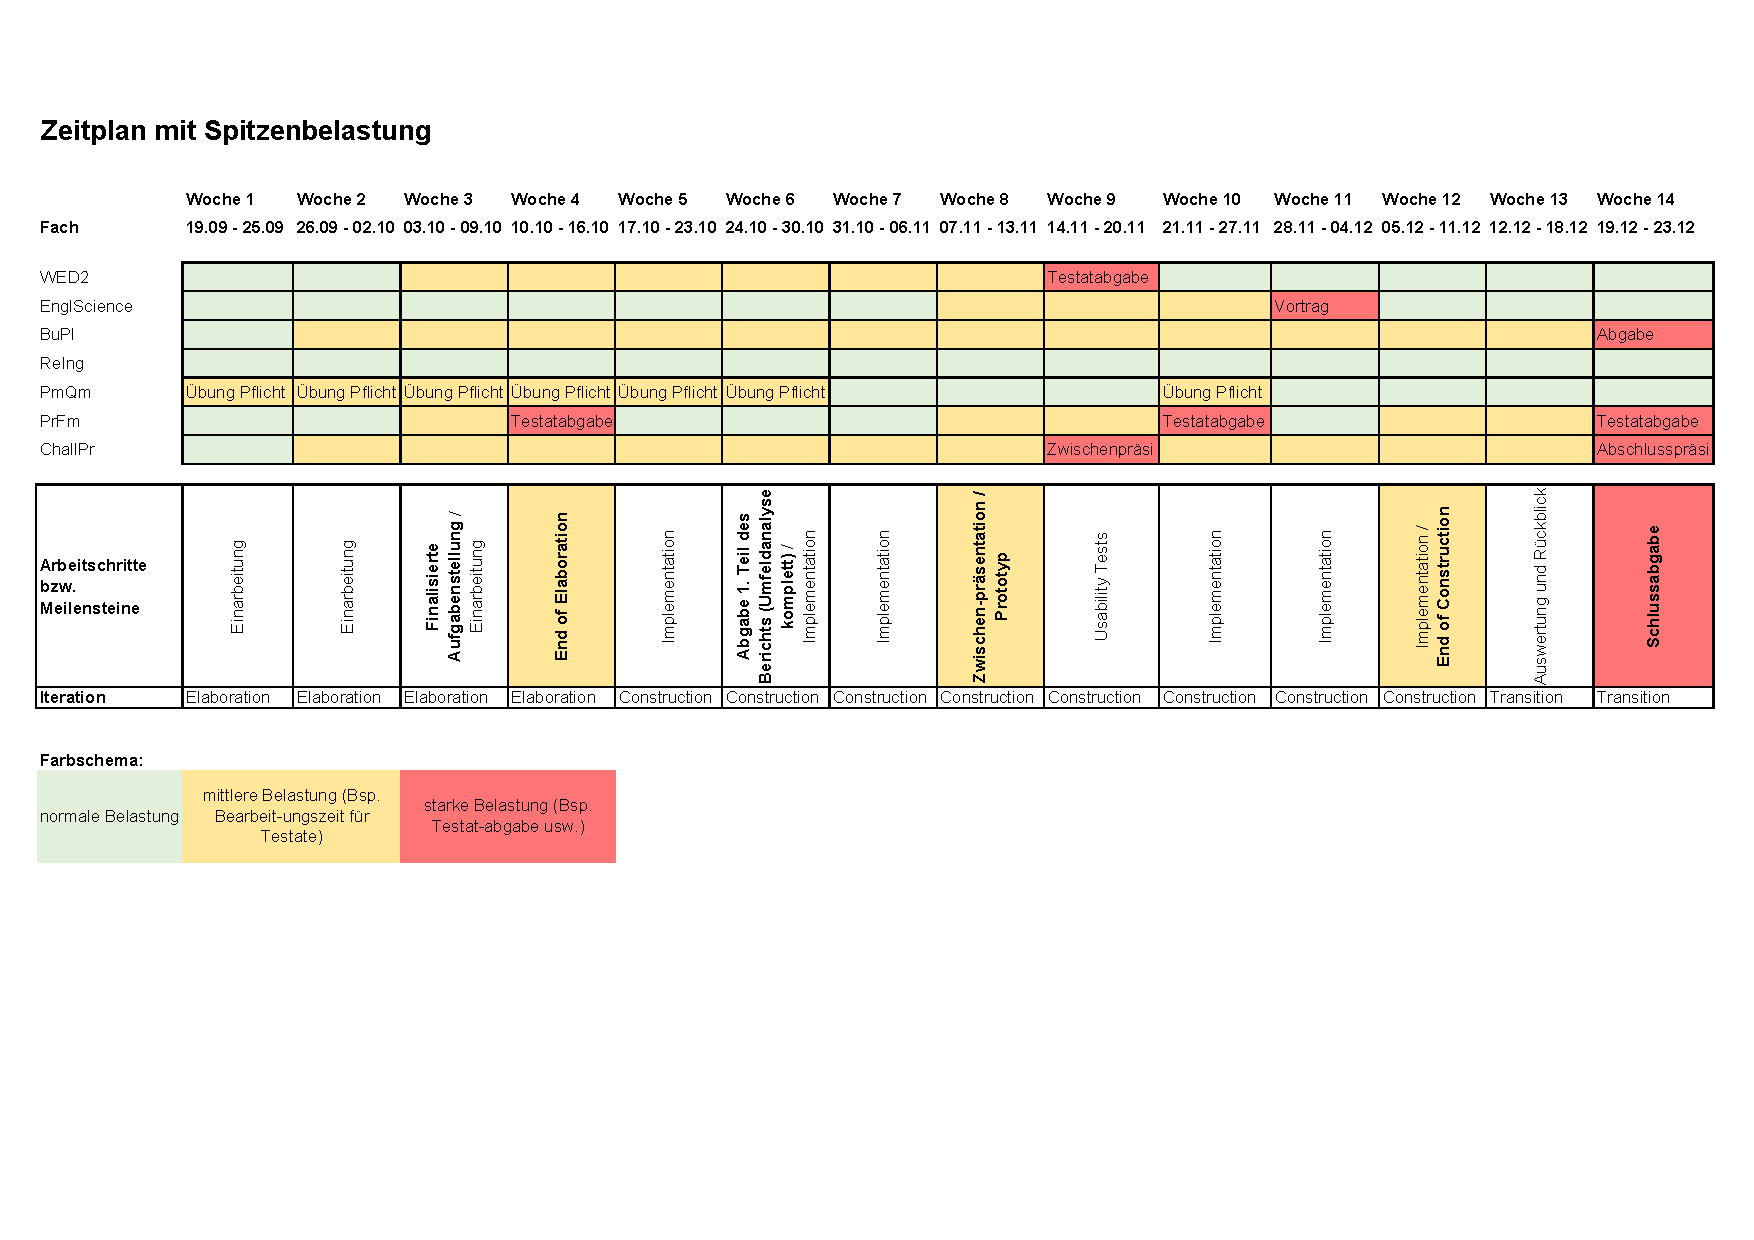
\includepdf[landscape=true]{PDFs/Zeitplan_Spitzenbelastung.pdf}
 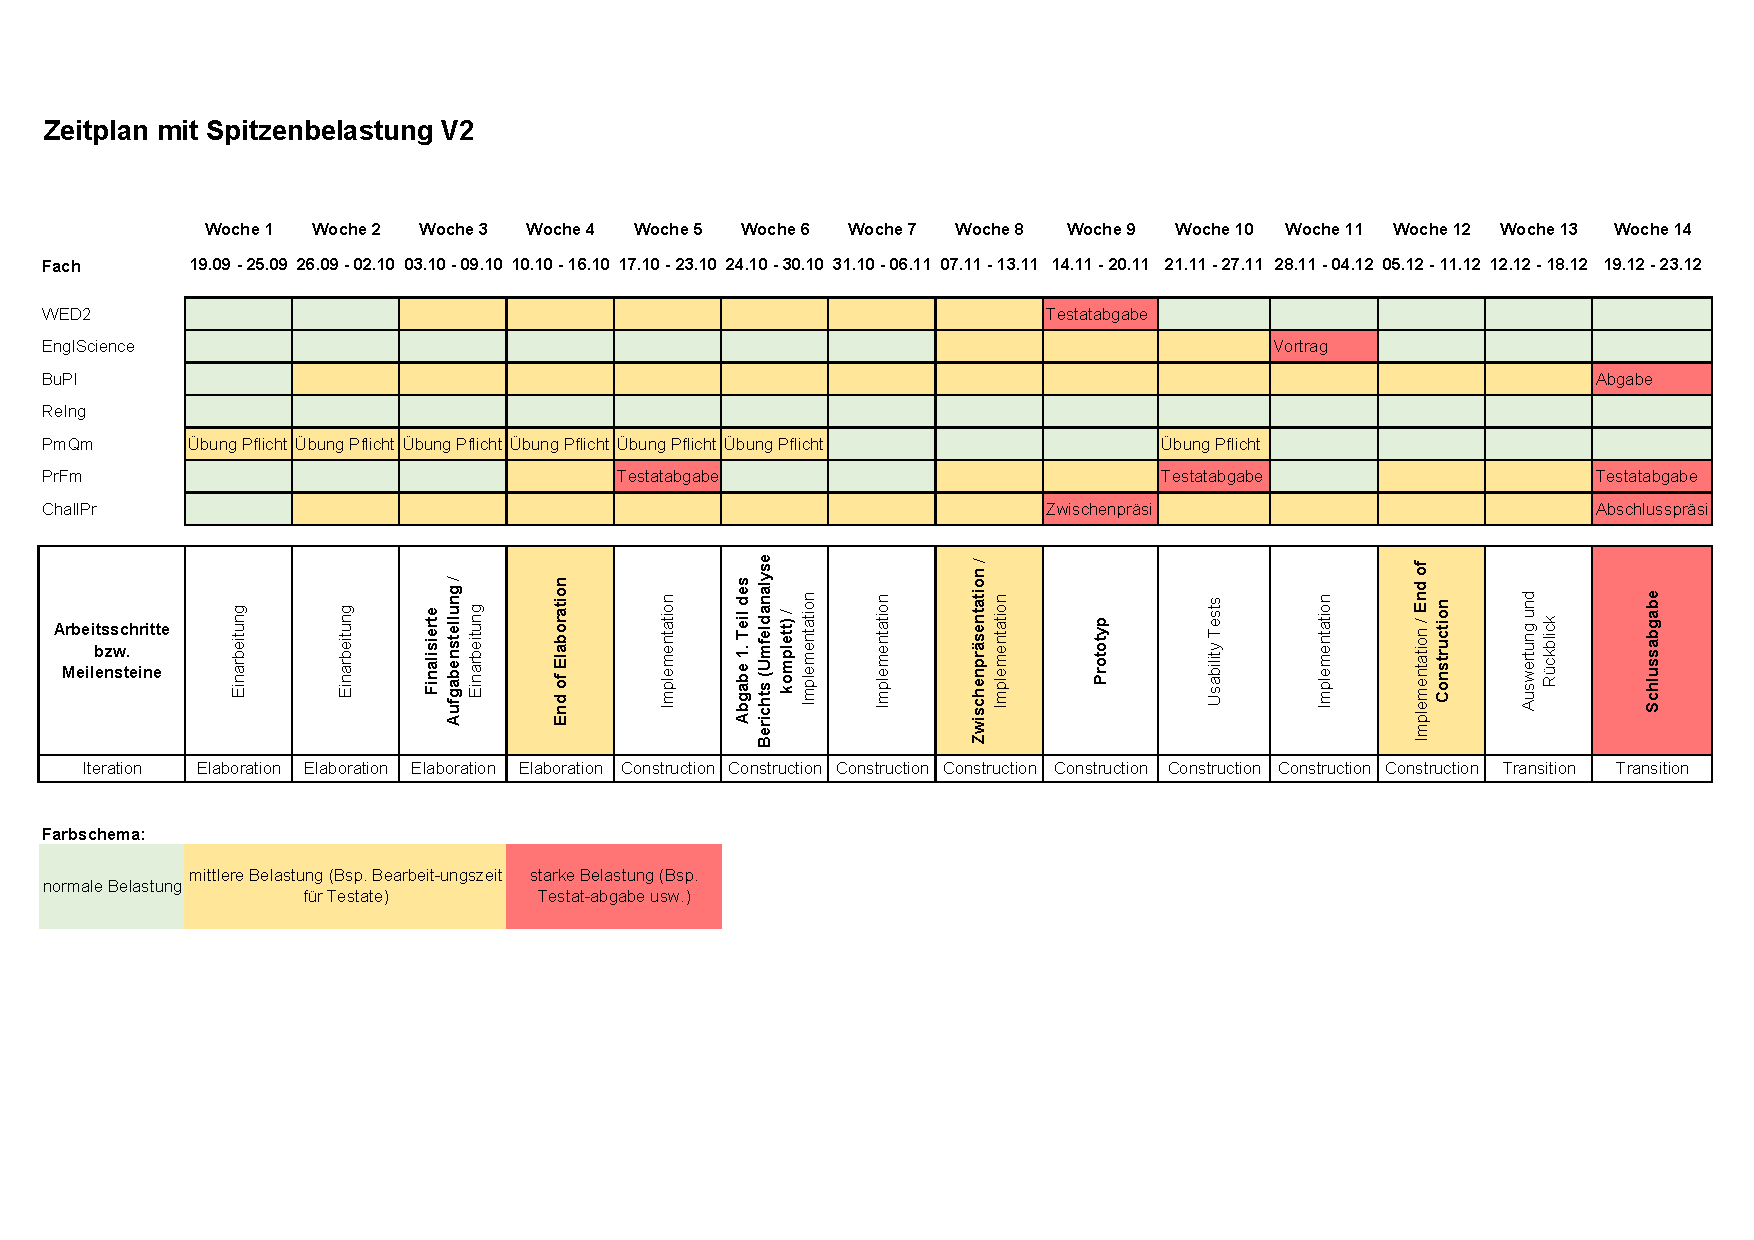
\includepdf[landscape=true]{PDFs/Zeitplan_SpitzenbelastungV2.pdf}
 
 
 \subsection{Meilensteine}
 %Die Meilensteine sollen konkret und messbar dargestellt werden.
 
 \begin{tabularx}{\linewidth}{|X|c|X|}
 	\hline
 	\textbf{Meilenstein} & \textbf{Datum} & \textbf{Beschreibung} \\
 	\hline
 	Finalisierte Aufgabenstellung & 09.10.2016 & Herr Heinzmann hat die zu erledigenden Arbeiten in einer Aufgabenstellung zusammengestellt und an die Studenten abgegeben. \\
 	\hline
 	End of Elaboration & 16.10.2016 & Die Umfeldanalyse ist abgeschlossen und es ist bekannt, welche Arbeiten im Rahmen der Studienarbeit angegangen werden. \\
 	\hline
 	Erster Teil des Berichts komplett & 30.10.2016 & Die Ergebnisse der Analyse-Phase sind vollständig niedergeschrieben, damit Herr Heinzmann diese gegenlesen kann. \\
 	\hline
 	Zwischenpräsentation & 13.11.2016 & Die bisher erarbeiteten Ergebnisse wurden Herrn Heinzmann als Vortrag präsentiert. \\
 	\hline
 	Erster Prototyp & 13.11.2016 & Die Code-Änderungen für eine verbesserte Usability wurden vollständig implementiert, damit in der Folgewoche die zweiten Usability-Tests durchgeführt werden können. \\
 	\hline
 	End of Construction & 11.12.2016 & Alle Änderungen am Code wurden implementiert, sodass dieser wieder auf den cnlab-Server übertragen werden kann. \\
 	\hline
 	Schlussabgabe & 23.12.2016 & Alle Dokumente wurden abgabekonform erstellt, die Dokumentation gebunden, der Code auf CD gebrannt und alles an Herrn Heinzmann abgegeben. \\
 	\hline
 \end{tabularx}
 
 
 
 \section{Zeiterfassung}
 Für alle Arbeiten werden in Redmine Arbeitspakete erfasst. Sofort nachdem ein Paket bearbeitet wurde, wird die Zeit darauf verbucht. Da alle Pakete einer Kategorie zugeordnet sind, kann am Ende des Projekts genau festgestellt werden, wie viel Zeit beispielsweise für alle Dokumentationen aufgewendet wurde.
 
 Die bereits erfassten Pakete sowie deren Fortschritt sind auf den folgenden Seiten abgebildet:
 
 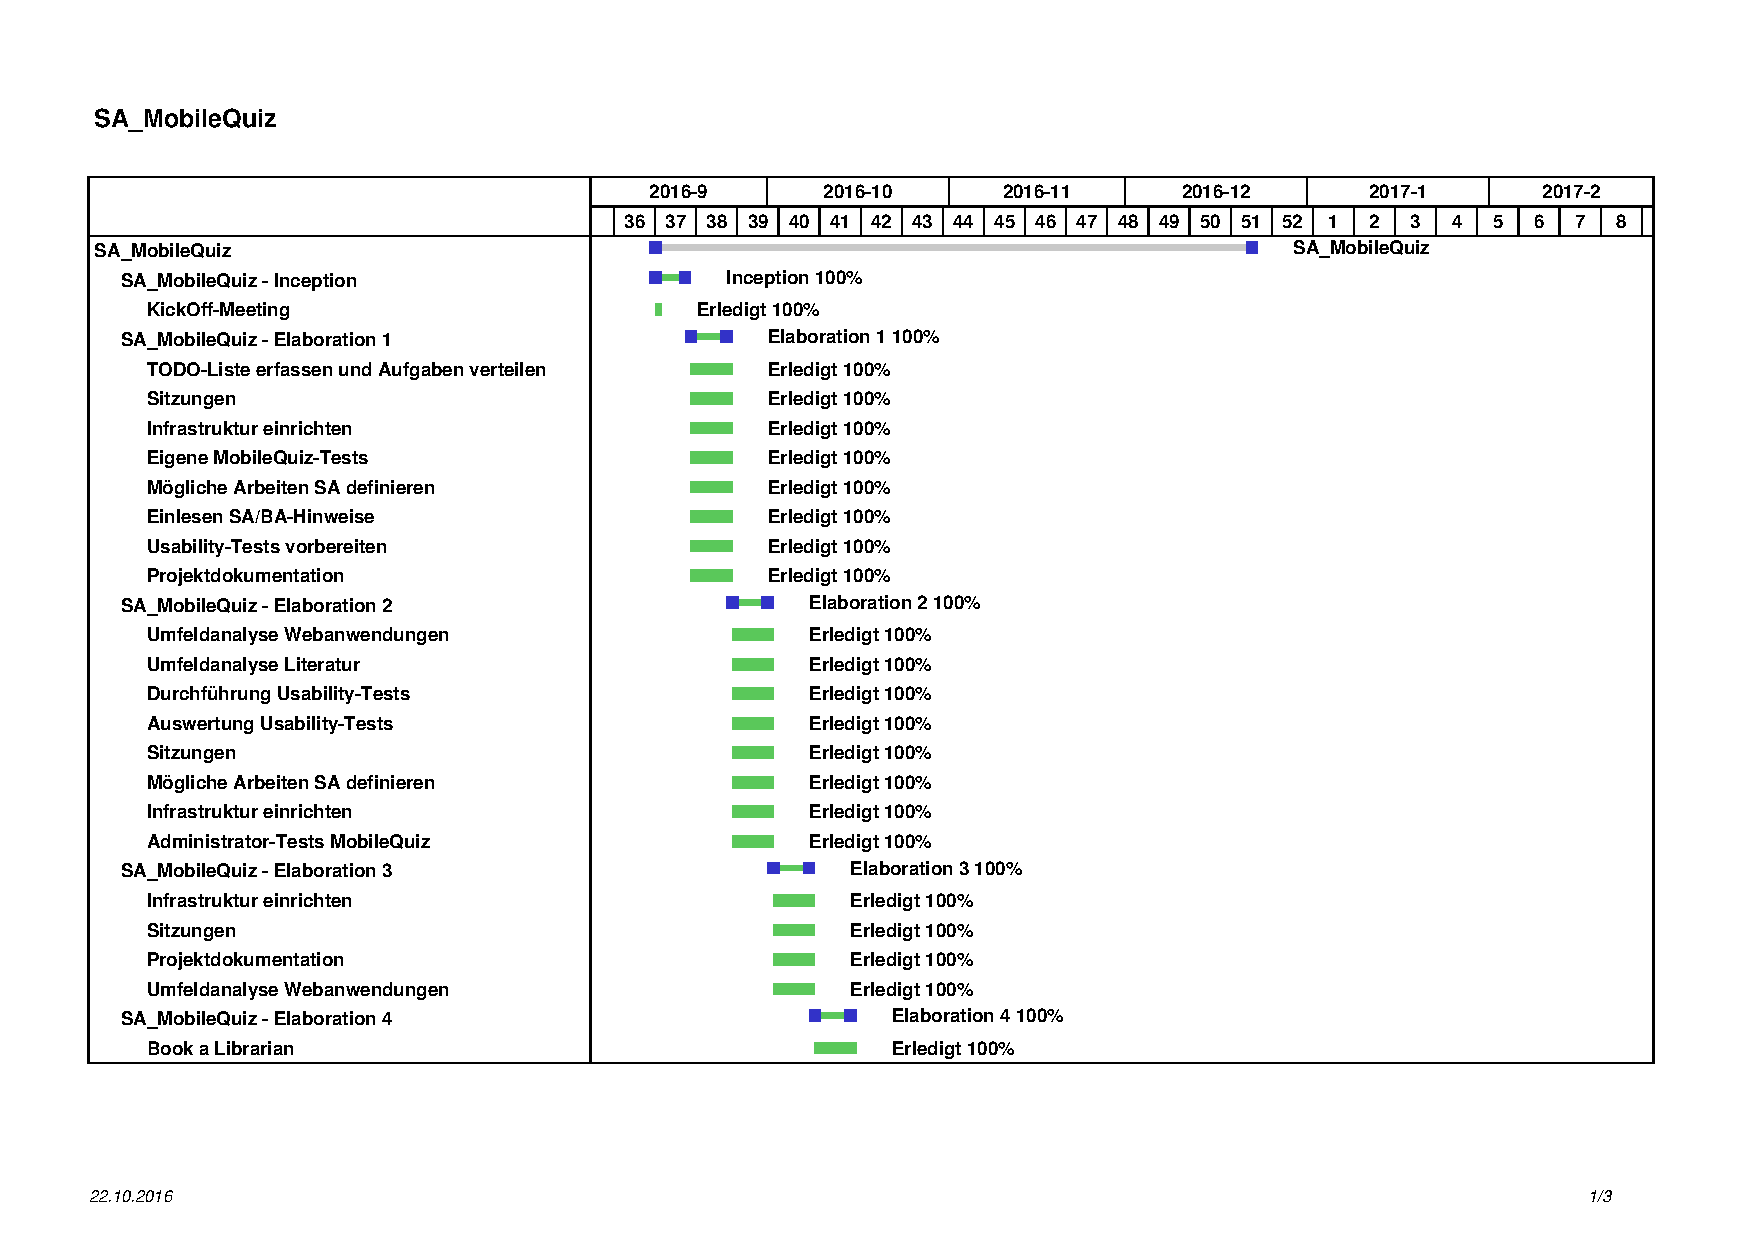
\includepdf[landscape=true,pages={1-3}]{PDFs/sa_mobilequiz-gantt_22-10-2016.pdf}